\documentclass[a4paper]{article}
\usepackage{amsmath,amssymb,float,geometry,graphicx,minted,pgfplots,tikz,xcolor}
% \captionsetup[figure]{labelsep=period}
% \captionsetup[table]{labelsep=period}
\geometry{left=3.5cm,right=3.5cm,top=3.3cm,bottom=3.3cm}
\definecolor{bg}{rgb}{0.95,0.95,0.95}
\pgfplotsset{compat=1.17}
\renewcommand\thesection{\arabic{section}}
% \usetikzlibrary {fixedpointarithmetic}
% \usetikzlibrary {fpu}
\usetikzlibrary {datavisualization}
\begin{document}
\begin{center}
\huge
\textbf{VE320\\Intro to Semiconductor Devices\\}
\Large
\vspace{30pt}
\uppercase{Homework 3}\\
\vspace{5pt}\today\\
\vspace{5pt}
Yihua Liu 518021910998
\vspace{5pt}
\rule[-10pt]{.97\linewidth}{0.05em}
\end{center}
1. (a) The density of states in the conduction band is
$$g_c(E)=\frac{4\pi(2m_n^*)^{3/2}}{h^3}\sqrt{E-E_c}.$$
Since $E=E_c+kT$,
$$g_c(E)=\frac{4\pi(2m_n^*)^{3/2}}{h^3}\sqrt{kT}.$$
The density of states in the valence band is
$$g_v(E)=\frac{4\pi(2m_p^*)^{3/2}}{h^3}\sqrt{E_v-E}.$$
Since $E=E_v-kT$,
$$g_v(E)=\frac{4\pi(2m_p^*)^{3/2}}{h^3}\sqrt{kT}.$$
The ratio of the density of states in the conduction band at $E=E_c+kT$ to the density of states in the valence band at $E=E_v-kT$ is
$$\frac{g_c(E)}{g_v(E)}=\frac{\frac{4\pi(2m_n^*)^{3/2}}{h^3}\sqrt{kT}}{\frac{4\pi(2m_p^*)^{3/2}}{h^3}\sqrt{kT}}=\bigg(\frac{m_n^*}{m_p^*}\bigg)^{3/2}.$$
According to textbook page 83 Table 4.1, we have $m_n^*/m_0=1.08$ and $m_p^*/m_0=0.56$ for Si. Thus, the ratio of the density of states in the conduction band at $E=E_c+kT$ to the density of states in the valence band at $E=E_v-kT$ is
$$\frac{g_c(E)}{g_v(E)}=\bigg(\frac{1.08}{0.56}\bigg)^{3/2}=2.678.$$
(b) For GaAs, $m_n^*/m_0=0.067$ and $m_p^*/m_0=0.48$. Thus, the ratio of the density of states in the conduction band at $E=E_c+kT$ to the density of states in the valence band at $E=E_v-kT$ is
$$\frac{g_c(E)}{g_v(E)}=\bigg(\frac{0.067}{0.48}\bigg)^{3/2}=0.0521.$$

2. (a) The probability of a state being occupied by an electron in the conduction band is
$$f_F(E)=\frac{1}{1+\exp{\big(\frac{E-E_F}{kT}\big)}}.$$
We have $E_c-E_F=0.30$ eV and $T=300$ K. Thus, The probability of a state being occupied by an electron in the conduction band is
$$f_F(E)=\frac{1}{1+\exp{\big(\frac{0.30\times1.602176565\times10^{-19}+x}{1.3806488\times10^{-23}\times300}\big)}}$$
over the range $E_c\leq E\leq E_c+2\times1.3806488\times10^{-23}\times300$ where $x=E-E_c$ over the range $0\leq x\leq0.05170399431$ eV.

The graph of $f_F(E)$ is shown in Figure 1.
% \begin{tikzpicture}
    % \draw[very thin,color=gray] (-0.1,-1.1) grid (3.9,3.9);
    % \draw[->] (-0.2,0) -- (4.2,0) node[right] {$E$ (eV)};
    % \draw[->] (-0.2,0) -- (4.2,0) node[above] {$f_F$};
    % \pgfkeys{/pgf/fpu}
    % \begin{axis}[restrict y to domain=0:1e-5]
    % \begin{axis}[
        % xlabel={$E$ [V]},
        % ylabel={$f_F(E)$},
    % ]
        % \pgfkeys{/pgf/fpu,/pgf/fpu/output format=sci}
        % \addplot[domain=0.30*1.602176565*10^(-19):0.30*1.602176565*10^(-19)+2*1.3806488*10^(-23)*300,samples=1000] {1/(1+exp((\x-0.30*1.602176565*10^(-19))/(1.3806488*10^(-23)*300)))} node[pos=0.65,left] {$f_F(E)=\frac{1}{1+\exp{\big(\frac{E-E_F}{kT}\big)}}$};
    % \pgfkeys{/pgf/fpu=false}
    % \end{axis}
    % \datavisualization [
        % scientific axes=clean,
        % visualize as smooth line
    % ]
    % data [read from file=3-2(a).csv];
% \end{tikzpicture}
\begin{figure}[H]
    \centering
    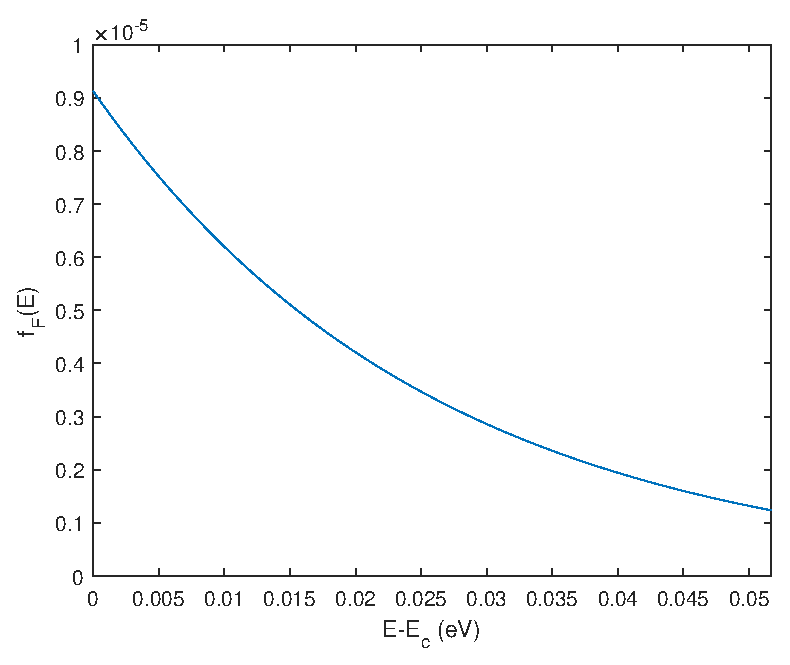
\includegraphics[width=1\textwidth]{3-2(a).eps}
    \caption{3-2(a).}
\end{figure}

(b) The probability of a state being empty by an electron in the valence band is
$$1-f_F(E)=1-\frac{1}{1+\exp{\big(\frac{E-E_F}{kT}\big)}}.$$
We have $E_F-E_v=0.25$ eV and $T=300$ K. Thus, The probability of a state being empty by an electron in the valence band is
$$f_F(E)=1-\frac{1}{1+\exp{\big(\frac{-0.25\times1.602176565\times10^{-19}+x}{1.3806488\times10^{-23}\times300}\big)}}$$
over the range $E_v-2\times1.3806488\times10^{-23}\times300\leq E\leq E_v$ where $x=E-E_v$ over the range $-0.05170399431\leq x\leq0$ eV.
\begin{figure}[H]
    \centering
    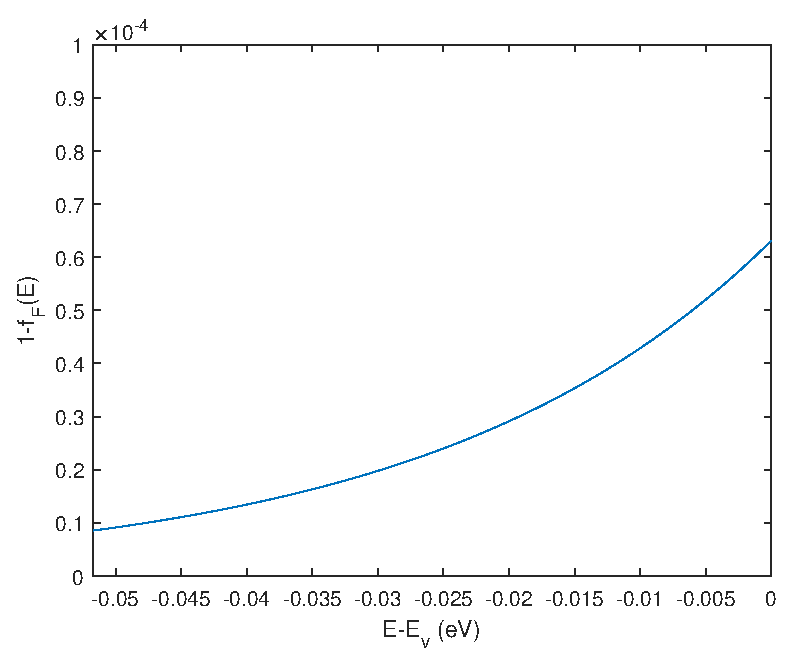
\includegraphics[width=1\textwidth]{3-2(b).eps}
    \caption{3-2(b).}
\end{figure}

3. (a) Since the probability is
$$f_F(E)=\frac{1}{1+\exp{\big(\frac{E-E_F}{kT}\big)}},$$
we have the temperature is
$$T=\frac{E-E_F}{k\ln{(\frac{1}{f_F}-1})}.$$
Substituting $10^{-8}$ for $f_F$ and $0.60$ eV for $E-E_F$, the temperature at which there is a $10^{-8}$ probability that an energy state 0.60 eV above the Fermi energy level is occupied by an electron is
$$T=\frac{0.6\times1.602176565\times10^{-19}}{1.3806488\times10^{-23}\times\ln{(\frac{1}{10^{-8}}-1})}=378.0\ \text{K}.$$

(b) Similarly, substituting $10^{-6}$ for $f_F$ and $0.60$ eV for $E-E_F$, the temperature at which there is a $10^{-8}$ probability that an energy state 0.60 eV above the Fermi energy level is occupied by an electron is
$$T=\frac{0.6\times1.602176565\times10^{-19}}{1.3806488\times10^{-23}\times\ln{(\frac{1}{10^{-6}}-1})}=504.0\ \text{K}.$$

4. (a) The position of the intrinsic Fermi level with respect to the center of the bandgap is:
$$E_{Fi}-E_\text{midgap}=\frac{3}{4}kT\ln{\bigg(\frac{m_p^*}{m_n^*}\bigg)}.$$
Therefore, the position of the intrinsic Fermi level with respect to the center of the bandgap at $T=300$ K is
$$E_{Fi}-E_\text{midgap}=\frac{3}{4}\times1.3806488\times10^{-23}\times300\ln{\bigg(\frac{0.70m_0}{1.21m_0}\bigg)}=-1.70\times10^{-21}\ \text{V}=-0.0106\ \text{eV}.$$
(b) Similarly, the position of the intrinsic Fermi level with respect to the center of the bandgap at $T=300$ K is
$$E_{Fi}-E_\text{midgap}=\frac{3}{4}\times1.3806488\times10^{-23}\times300\ln{\bigg(\frac{0.75m_0}{0.080m_0}\bigg)}=6.95\times10^{-21}\ \text{V}=-0.0434\ \text{eV}.$$

5. (a) The concentration of holes
$$p_0=N_v\exp{\bigg[\frac{-(E_F-E_v)}{kT}\bigg]}.$$
Thus, the expression for $E_F-E_v$ is
$$E_F-E_v=-kT\ln{\Big(\frac{p_0}{N_v}\Big)}.$$
Substituting $300$ K for $T$, $5\times10^{15}\ \text{cm}^{-3}$ for $p_0$, and $1.04\times10^{19}\ \text{cm}^{-3}$, we have
$$E_F-E_v=-1.3806488\times10^{-23}\times300\ln{\Big(\frac{5\times10^{15}}{1.04\times10^{19}}\Big)}=3.16\times10^{-20}\ \text{V}=0.198\ \text{eV}.$$

(b) Since the width of a forbidden energy band $E_g$ of silicon is 1.12 eV, we have
$$E_c-E_F=E_g-(E_F-E_v)=1.12-0.198=0.922\ \text{eV}.$$

(c) The concentration of electrons is
$$n_0=N_c\exp{\Big[\frac{-(E_c-E_F)}{kT}\Big]}=N_c\exp{\Big[-\Big(\frac{E_g}{kT}+\ln{\Big(\frac{p_0}{N_v}\Big)}\Big)\Big]}.$$
Substituting $2.8\times10^{19}\ \text{cm}^{-3}$ for $N_c$ and $300$ K for $T$,
$$n_0=2.8\times10^{19}\exp{\Big[-\Big(\frac{1.12\times1.602176565\times10^{-19}}{1.3806488\times10^{-23}\times300}+\ln{\Big(\frac{5\times10^{15}}{1.04\times10^{19}}\Big)}\Big)\Big]}=8.91\times10^{3}\ \text{cm}^{-3}.$$

(d) According to (c), $n_0<p_0$, so $\boxed{\text{hole}}$ is the majority carrier.

(e) The concentration of holes is
$$p_0=n_i\exp{\bigg[\frac{-(E_F-E_{Fi})}{kT}\bigg]}=n_i\exp{\bigg[\frac{E_{Fi}-E_F)}{kT}\bigg]},$$
thus,
$$E_{Fi}-E_F=kT\ln{\Big(\frac{p_0}{n_i}\Big)}.$$
According to Chapter 4 Section 4.1.3 of the textbook, there is discrepancy between the commonly accepted value of $n_i$ and the value of $n_i$ calculated from Equation (4.23) for $E_g=1.12$ eV, though we take the intrinsic carrier concentration $n_i$ of silicon as $1.5\times10^{10}\ \text{cm}^{-3}$. Therefore,
$$E_{Fi}-E_F=1.3806488\times10^{-23}\times300\times\ln{\Big(\frac{5\times10^{15}}{1.5\times10^{10}}\Big)}=5.27\times10^{-20}\ \text{V}=0.329\ \text{eV}.$$

6. (a) (i) The thermal equilibrium electron concentration is
$$n_0=\frac{N_d-N_a}{2}+\sqrt{\Big(\frac{N_d-N_a}{2}\Big)^2+n_i^2}.$$
Substituting $2\times10^{15}\ \text{cm}^{-3}$ for $N_d$, $0$ for $N_a$, and $2.4\times10^{13}\ \text{cm}^{-3}$ for $n_i$, the thermal equilibrium electron concentration is
$$n_0=\frac{2\times10^{15}}{2}+\sqrt{\Big(\frac{2\times10^{15}}{2}\Big)^2+(2.4\times10^{13})^2}=2.00\times10^{15}\ \text{cm}^{-3}.$$
The thermal equilibrium hole concentration is
$$p_0=\frac{n_i^2}{n_0}.$$
Substituting $2.4\times10^{13}\ \text{cm}^{-3}$ for $n_i$, the thermal equilibrium hole concentration is
$$p_0=\frac{(2.4\times10^{13})^2}{\frac{2\times10^{15}}{2}+\sqrt{\big(\frac{2\times10^{15}}{2}\big)^2+(2.4\times10^{13})^2}}=2.88\times10^{11}\ \text{cm}^{-3}.$$

(ii) The thermal equilibrium hole concentration is
$$p_0=\frac{N_a-N_d}{2}+\sqrt{\Big(\frac{N_a-N_d}{2}\Big)^2+n_i^2}.$$
Substituting $10^{16}\ \text{cm}^{-3}$ for $N_a$, $7\times10^{15}\ \text{cm}^{-3}$ for $N_d$, and $2.4\times10^{13}\ \text{cm}^{-3}$ for $n_i$, the thermal equilibrium hole concentration is
$$p_0=\frac{10^{16}-7\times10^{15}}{2}+\sqrt{\Big(\frac{10^{16}-7\times10^{15}}{2}\Big)^2+(2.4\times10^{13})^2}=3.00\times10^{15}\ \text{cm}^{-3}.$$
The thermal equilibrium electron concentration is
$$n_0=\frac{n_i^2}{p_0}.$$
Substituting $2.4\times10^{13}\ \text{cm}^{-3}$ for $n_i$, the thermal equilibrium electron concentration is
$$n_0=\frac{(2.4\times10^{13})^2}{\frac{10^{16}-7\times10^{15}}{2}+\sqrt{\big(\frac{10^{16}-7\times10^{15}}{2}\big)^2+(2.4\times10^{13})^2}}=1.92\times10^{11}\ \text{cm}^{-3}.$$

(b) (i) Similarly, substituting $2\times10^{15}\ \text{cm}^{-3}$ for $N_d$, $0$ for $N_a$, and $1.8\times10^{6}\ \text{cm}^{-3}$ for $n_i$, the thermal equilibrium electron concentration is
$$n_0=\frac{2\times10^{15}}{2}+\sqrt{\Big(\frac{2\times10^{15}}{2}\Big)^2+(1.8\times10^{6})^2}=2.00\times10^{15}\ \text{cm}^{-3}.$$
The thermal equilibrium hole concentration is
$$p_0=\frac{(1.8\times10^{6})^2}{\frac{2\times10^{15}}{2}+\sqrt{\big(\frac{2\times10^{15}}{2}\big)^2+(1.8\times10^{6})^2}}=1.62\times10^{-3}\ \text{cm}^{-3}.$$

(ii) Similarly, substituting $10^{16}\ \text{cm}^{-3}$ for $N_a$, $7\times10^{15}\ \text{cm}^{-3}$ for $N_d$, and $1.8\times10^{6}\ \text{cm}^{-3}$ for $n_i$, the thermal equilibrium hole concentration is
\[
    \begin{aligned}
        p_0&=\frac{N_a-N_d}{2}+\sqrt{\Big(\frac{N_a-N_d}{2}\Big)^2+n_i^2}\\
        &=\frac{10^{16}-7\times10^{15}}{2}+\sqrt{\Big(\frac{10^{16}-7\times10^{15}}{2}\Big)^2+(1.8\times10^{6})^2}\\
        &=3.00\times10^{15}\ \text{cm}^{-3}.
    \end{aligned}
\]
The thermal equilibrium electron concentration is
$$n_0=\frac{n_i^2}{p_0}=\frac{(2.4\times10^{13})^2}{\frac{10^{16}-7\times10^{15}}{2}+\sqrt{\big(\frac{10^{16}-7\times10^{15}}{2}\big)^2+(1.8\times10^{6})^2}}=1.08\times10^{-3}\ \text{cm}^{-3}.$$

(c) The minority carrier concentration, i.e., the concentration of electrons in the conduction band decreases below the intrinsic carrier concentration as we add acceptor impurity atoms. At the same time, the majority carrier hole concentration increases above the intrinsic carrier concentration as we add acceptor atoms. As we add acceptor impurity atoms and the corresponding acceptor holes, there is a redistribution of holes among available energy states. A few of the acceptor holes will rise into the empty states in the conduction band and in doing so will annihilate some of the intrinsic electrons. The minority carrier electron concentration will therefore decrease.

7. (a) Since boron atoms are acceptor and arsenic atoms are donor, the concentration of boron atoms is $N_a=3\times10^{16}\ \text{cm}^{-3}$ that is higher than the concentration of arsenic atoms $N_d=1.5\times10^{16}\ \text{cm}^{-3}$, the material is $\boxed{\text{p type}}$.

The thermal equilibrium concentrations of majority carriers is
$$p_0=N_a-N_d=3\times10^{16}-1.5\times10^{16}=1.5\times10^{16}\ \text{cm}^{-3}.$$
The thermal equilibrium concentrations of minority carriers is
$$n_0=\frac{n_i^2}{p_0}=\frac{(1.5\times10^{10})^2}{1.5\times10^{16}}=1.5\times10^{4}\ \text{cm}^{-3}.$$

(b) To make holes to be the majority carrier and the thermal equilibrium concentration to be $p_0=5\times10^{16}\ \text{cm}^{-3}$, boron atoms must be added.

We have
$$n_0+N_a=p_0+N_d.$$
Since $n_0\ll p_0$, we can ignore $n_0$. $N_a$ here is the sum of the original and the added concentration of acceptor atoms. Denote the concentration of the acceptor atoms to be added as $N_A'$, then we have
$$N_a'=p_0+N_d-N_A.$$
Substituting $1.5\times10^{16}\ \text{cm}^{-3}$ for $N_d$, $3\times10^{16}\ \text{cm}^{-3}$ for $N_a$, and $5\times10^{16}\ \text{cm}^{-3}$ for $p_0$, the concentration of impurity atoms must be added is
$$N_a'=5\times10^{16}+1.5\times10^{16}-3\times10^{16}=3.5\times10^{16}\ \text{cm}^{-3}.$$
The new value of $n_0$ is
$$n_0=\frac{n_i^2}{p_0}=\frac{(1.5\times10^{10})^2}{5\times10^{16}}=4.5\times10^{3}\ \text{cm}^{-3}.$$

8. (a) Since the silicon device is only doped with donor impurity atoms, we have the concentration of electrons is
$$n_0=\frac{N_d}{2}+\sqrt{\Big(\frac{N_d}{2}\Big)^2+n_i^2}.$$
Since the intrinsic carriers must contribute no more than 5 percent to the total electron concentration, when the temperature is at the maximum,
$$n_i=0.05n_0.$$
Therefore, the concentration of electrons is
$$n_0=\frac{10^{15}}{2}+\sqrt{\Big(\frac{10^{15}}{2}\Big)^2+(0.05n_0)^2}.$$
Solving the equation above, we have the majority carrier electron is
$$n_0=1.00\times10^{15}\ \text{cm}^{-3},$$
thus, the concentration of the intrinsic carrier is
$$n_i=5.01\times10^{13}\ \text{cm}^{-3}.$$
We have
$$n_i^2=N_cN_v\exp{\Big(\frac{-E_g}{kT}\Big)},$$
so
$$T=\frac{-E_g}{k\ln{\Big(\frac{n_i^2}{N_cN_v}\Big)}}.$$
Substituting $5.01\times10^{13}\ \text{cm}^{-3}$ for $n_i$, $2.8\times10^{19}\ \text{cm}^{-3}$ for $N_c$, $1.04\times10^{19}\ \text{cm}^{-3}$ for $N_v$, and $1.12$ eV for $E_g$, the maximum temperature that the device may operate is
$$T=\frac{-1.12\times1.602176565\times10^{-19}}{1.3806488\times10^{-23}\times\ln{\Big(\frac{n_i^2}{2.8\times10^{19}\times1.04\times10^{19}}\Big)}}=510\ \text{K}.$$

(b) We have
$$E_c-E_F=kT\ln{\Big(\frac{N_c}{N_d}\Big)}.$$
Therefore,
$$\Delta(E_c-E_F)=k\Delta T\ln{\Big(\frac{N_c}{N_d}\Big)}.$$
Substituting $2.8\times10^{19}\ \text{cm}^{-3}$ for $N_c$ and $10^{15}\ \text{cm}^{-3}$ for $N_d$, the change in $E_c-E_F$ from the $T=300$ K value to the maximum temperature value determined in part (a) is
$$\Delta(E_c-E_F)=1.3806488\times10^{-23}\times(510-300)\times\ln{\Big(\frac{2.8\times10^{19}}{10^{15}}\Big)}=2.97\times10^{-20}\ \text{J}=0.185\ \text{eV}.$$

(c) As the temperature increases, the intrinsic carrier concentration increases. Therefore, the Fermi level is $\boxed{\text{closer}}$ to the intrinsic value at the higher temperature.

9. (a) The position of the intrinsic Fermi energy level with respect to the center of the bandgap is
$$E_{Fi}-E_\text{midgap}=\frac{3}{4}kT\ln{\bigg(\frac{m_p^*}{m_n^*}\bigg)}.$$
Substituting 10 for $\frac{m_p^*}{m_n^*}$, 300 K for $T$, the position of the intrinsic Fermi energy level with respect to the center of the bandgap is
$$E_{Fi}-E_\text{midgap}=\frac{3}{4}\times1.3806488\times10^{-23}\times300\times\ln{10}=7.15\times10^{-21}\ \text{V}=0.0446\ \text{eV}.$$

(b) (i) Since the Fermi energy level is lower, $\boxed{\text{acceptor}}$ atoms are added.

(ii) The concentration of impurity atoms added is
$$p_0=n_i\exp{\Big(\frac{E_{Fi}-E_F}{kT}\Big)}.$$
According to (a),
$$E_{Fi}-E_F=0.45+0.0446=0.4946\ \text{eV}.$$
Substituting $1\times10^5\ \text{cm}^{-3}$ for $n_i$, $0.4946\ \text{eV}$ for $E_{Fi}-E_F$, and 300 K for $T$, the concentration of impurity atoms added is
$$p_0=10^5\exp{\Big(\frac{0.4946\times1.602176565\times10^{-19}}{1.3806488\times10^{-23}\times300}\Big)}=2.04\times10^{13}\ \text{cm}^{-3}.$$

10. (a) The donor concentrations is
$$N_d=0.05\times7\times10^{15}=3.5\times10^{14}\ \text{cm}^{-3}.$$
The accept concentration is
$$N_a=0.95\times7\times10^{15}=6.65\times10^{15}\ \text{cm}^{-3}.$$

(b) Since $N_a>N_d$, the material is $\boxed{\text{p type}}$.

(c) The hole concentration is
$$p_0=N_a-N_d.$$
Substituting $6.65\times10^{15}\ \text{cm}^{-3}$ for $N_a$ and $3.5\times10^{14}\ \text{cm}^{-3}$ for $N_d$, the hole concentration is
$$p_0=6.65\times10^{15}-3.5\times10^{14}=6.3\times10^{15}\ \text{cm}^{-3}.$$
The electron concentration is
$$n_0=\frac{n_i^2}{p_0}.$$
Substituting $6.3\times10^{15}\ \text{cm}^{-3}$ for $p_0$ and $1.8\times10^{6}\ \text{cm}^{-3}$ for $n_i$, the electron concentration is
$$n_0=\frac{(1.8\times10^{6})^2}{6.3\times10^{15}}=5.14\times10^{-4}\ \text{cm}^{-3}.$$

(d) We have
$$E_{Fi}-E_F=kT\ln{\Big(\frac{p_0}{n_i}\Big)}.$$
Substituting $6.3\times10^{15}\ \text{cm}^{-3}$ for $p_0$, $1.8\times10^{6}\ \text{cm}^{-3}$ for $n_i$, and 300 K for $T$, the position of the Fermi level with respect to $E_{Fi}$ is
$$E_{Fi}-E_F=1.3806488\times10^{-23}\times300\times\ln{\Big(\frac{6.3\times10^{15}}{1.8\times10^{6}}\Big)}=9.10\times10^{-20}\ \text{V}=0.568\ \text{eV}.$$

11. (a) We have
\begin{equation}
    n_i^2=N_cN_v\exp{\Big(\frac{-E_g}{kT}\Big)},
\end{equation}
thus
$$n_i=\sqrt{N_cN_v\exp{\Big(\frac{-E_g}{kT}\Big)}}.$$
At $T=300$ K, substituting $2.0\times10^{19}\ \text{cm}^{-3}$ for $N_c$, $1\times10^{19}\ \text{cm}^{-3}$ for $N_v$, 1.10 eV for $E_g$, and 300 K for $T$, the intrinsic carrier concentration is
$$n_i=\sqrt{2.0\times10^{19}\times10^{19}\exp{\Big(\frac{-1.10\times1.602176565\times10^{-19}}{1.3806488\times10^{-23}\times300}\Big)}}=8.15\times10^{9}\ \text{cm}^{-3}.$$
The donor concentration $N_d=10^{14}\ \text{cm}^{-3}$ which is much larger than $n_i$, so the electron concentration is
$$n=N_d=10^{14}\ \text{cm}^{-3}.$$
The electric-current density is
$$J=e\mu_nnE.$$
Substituting 1000 $\mathrm{cm}^2/\text{V}\cdot\text{s}$ for $\mu_n$, $10^{14}\ \text{cm}^{-3}$ for $n$, and 100 V/cm for $E$, the electric-current density is
$$J=1.602176565\times10^{-19}\times1000\times10^{14}\times100=1.60\ \text{A}/\mathrm{cm}^2.$$

(b) To make this current increase by 5 percent, the intrinsic carrier concentration $n'$ would increase to $1.05n=1.05\times10^{14}\ \text{cm}^{-3}$. To derive the intrinsic carrier concentration $n_i$, we have
$$n_0=\frac{N_d}{2}+\sqrt{\Big(\frac{N_d}{2}\Big)^2+n_i^2},$$
thus,
$$n_i=\sqrt{n_0^2-n_0N_d}.$$
Substituting $1.05\times10^{14}\ \text{cm}^{-3}$ for $n_0$ and $10^{14}\ \text{cm}^{-3}$ for $N_d$, we have
$$n_i=\sqrt{(1.05\times10^{14})^2-1.05\times10^{14}\times10^{14}}=2.29\times10^{13}\ \text{cm}^{-3}.$$
Using Eq. (1), substituting 1.10 eV for $E_g$, $2\times10^{19}(T/300)^{3/2}\ \text{cm}^{-3}$ for $N_c$, and $1\times10^{19}(T/300)^{3/2}\ \text{cm}^{-3}$ for $N_v$, we have
$$(1.05\times10^{14})^2-1.05\times10^{14}\times10^{14}=2\times10^{38}\Big(\frac{T}{300}\Big)^3\exp{\Big(\frac{-1.10\times1.602176565\times10^{-19}}{1.3806488\times10^{-23}\times T}\Big)}.$$
Solving the equation, the temperature at which this current will increase by 5 percent is
$$T=457\ \text{K}.$$

12. The intrinsic carrier concentration
$$n_i=p_i=\sqrt{N_cN_v\exp{\Big(\frac{-E_g}{kT}\Big)}}=\sqrt{2.912\exp{\Big(\frac{-1.12e}{kT}\Big)}}\times10^{19}\Big(\frac{T}{300}\Big)^{3/2}.$$
The intrinsic conductivity is
\[
    \begin{aligned}
        \sigma&=e(\mu_nn+\mu_pp)\\
        &=e\sqrt{2.912\exp{\Big(\frac{-1.12e}{kT}\Big)}}\times10^{19}\Big(\frac{T}{300}\Big)^{3/2}\times1830\Big(\frac{T}{300}\Big)^{-3/2}\\
        &=1.83e\times10^{22}\sqrt{2.912\exp{\Big(\frac{-1.12e}{kT}\Big)}}
    \end{aligned}
\]
The graph of the intrinsic conductivity as a function of $T$ over the range $200\leq T\leq600$ K is shown in Figure 3.
\begin{figure}[H]
    \centering
    \includegraphics[width=1\textwidth]{3-12.eps}
    \caption{3-12.}
\end{figure}

13. (a) The electron field is
$$E_x=-\Big(\frac{kT}{e}\Big)\frac{1}{N_d(x)}\frac{\mathrm{d}N_d(x)}{\mathrm{d}x}.$$
Since $N_d(x)=N_{d0}e^{-x/L}=10^{16}e^{-x/L}$ and its derivative is $-\frac{10^{16}}{L}e^{-x/L}$, the electron field as a function of $x$ for $0\leq x\leq L$ is
\[
    \begin{aligned}
        E_x&=-\Big(\frac{1.3806488\times10^{-23}\times300}{1.602176565\times10^{-19}}\Big)\frac{1}{10^{16}e^{-x/L}}\frac{-10^{16}}{L}e^{-x/L}\\
        &=\frac{1.3806488\times10^{-23}\times300}{1.602176565\times10^{-19}\times10^{-5}}\\
        &=2.59\times10^{3}\ \text{V/m}.
    \end{aligned}
\]

(b) Since the electron field is a constant, the potential difference is
$$V=E_xL.$$
Therefore, the potential difference between $x=0$ and $x=L$ is
$$V=\frac{1.3806488\times10^{-23}\times300}{1.602176565\times10^{-19}}=2.59\times10^{-2}\ \text{V}.$$

14. (a) (i) Using the Einstein relation
$$\frac{D_n}{\mu_n}=\frac{kT}{e},$$
we have the diffusion coefficient is
$$D_n=\frac{kT\mu_n}{e}.$$
Substituting 300 K for $T$ and $1150\ \mathrm{cm}^2/\mathrm{V\cdot s}$ for $\mu_n$, the diffusion coefficient is
$$D_n=\frac{1.3806488\times10^{-23}\times300\times1150}{1.602176565\times10^{-19}}=29.7\ \mathrm{{cm}^2/s}.$$

(ii) Similarly, substituting 300 K for $T$ and $6200\ \mathrm{cm}^2/\mathrm{V\cdot s}$ for $\mu_n$, the diffusion coefficient is
$$D_n=\frac{1.3806488\times10^{-23}\times300\times1150}{1.602176565\times10^{-19}}=160\ \mathrm{{cm}^2/s}.$$

(b) (i) Using the Einstein relation
$$\frac{D_p}{\mu_p}=\frac{kT}{e},$$
we have the hole mobility is
$$\mu_p=\frac{eD_p}{kT}.$$
Substituting 300 K for $T$ and $8\ \mathrm{cm}^2/\mathrm{s}$ for $D_p$, the hole mobility is
$$\mu_p=\frac{1.602176565\times10^{-19}\times8}{1.3806488\times10^{-23}\times300}=309\ \mathrm{{cm}^2/V\cdot s}.$$

(ii) Similarly, substituting 300 K for $T$ and $8\ \mathrm{cm}^2/\mathrm{s}$ for $D_p$, the hole mobility is
$$\mu_p=\frac{1.602176565\times10^{-19}\times35}{1.3806488\times10^{-23}\times300}=1.35\times10^{3}\ \mathrm{{cm}^2/V\cdot s}.$$

15. The electron difference current density is
$$J_{nx|\text{dif}}=eD_n\frac{dn}{dx}.$$
Since the steady-state electron distribution in silicon can be approximated by a linear function of $x$, we can calculate the derivative by
$$\frac{dn}{dx}=\frac{n(0.012)-n(0)}{0.012-0}=-1.25\times10^{18}\ \text{cm}^{-4}.$$
Substituting $27\ \mathrm{{cm}^2/s}$ for $D_n$, the electron difference current density is
$$J_{nx|\text{dif}}=1.602176565\times10^{-19}\times27\times(-1.25\times10^{18})=-5.41\ \mathrm{A/{cm}^2}.$$
\section*{Appendices}
\renewcommand\thesubsection{\Alph{subsection}.}
\subsection{MATLAB Code for 3-2}
\inputminted[frame=single,bgcolor=bg,breaklines,breakanywhere]{matlab}{P3_2.m}
\subsection{Mathematica Code for 3-12}
\inputminted[frame=single,bgcolor=bg,breaklines,breakanywhere]{mathematica}{hw3.nb}
\end{document}